\documentclass[12pt,a4paper]{report}

\usepackage[utf8]{inputenc}
\usepackage[english]{babel}
\usepackage{amsmath}
\usepackage{amsfonts}
\usepackage{amssymb}
\usepackage{graphicx}
\usepackage{hyperref}
\usepackage{todonotes}
\usepackage{xcolor}
\usepackage{listings}
\usepackage{authblk}
\usepackage{algorithm, algpseudocode}

\newcommand{\ie}{\textit{i.e.}}
%customized todo
\definecolor{lightgreen}{rgb}{0.8,1.0,0.8}
\definecolor{red}{rgb}{0.8,0,0}
\definecolor{green}{rgb}{0,0.8,0}
\definecolor{blue}{rgb}{0,0,1}
\newcommand{\mytodo}[1]{\todo[inline,color=lightgreen]{TODO: #1}}
\newcommand{\myremark}[1]{\todo[inline, color=lightgreen]{\textbf{Remark:} #1}}

\title{The VNN-LIB standard for benchmarks\\2022}

\author[1]{Stefano Demarchi}
\author[2]{Dario Guidotti}
\author[2]{Luca Pulina}
\author[1]{Armando Tacchella}

\affil[1]{University of Genoa, Viale Causa 13, 16145 Genoa, Italy}
\affil[2]{University of Sassari, Via Roma 151, 07100 Sassari, Italy}
  
\begin{document}

\maketitle

\begin{abstract}
  The purpose of this document is to present the first version of the
  standard for neural network verification benchmarks, expressed as
  VNN-LIB. This standard builds on the Open Neural Network Exchange 
  (ONNX) format for model description, and on the Satisfiabily Modulo
  Theories Library (SMT-LIB) format for the property specification. 
  Throughout the document we will refer to the combination of model 
  and property description formats as the \emph{VNN-LIB format}.
\end{abstract}


\section*{Introduction}

In the last years the community of neural networks verification has
been growing larger and larger: after three years of the official
competition VNN-COMP we identified the needs and patterns that can
help people designing and improving their benchmarks.

This document is structured as follows. In Chapter~\ref{sec:model} we
present the guidelines for the model specification language, i.e., how
to describe the neural network for verification purposes and which 
operators are either supported, to be supported or discouraged; in
Chapter~\ref{sec:property} we present the guidelines for the property
specification language, i.e., how to specify the requirements that the
neural network ought to satisfy. Finally, in Section~\ref{sec:examples} 
we present some examples of benchmarks to further illustrate the
capabilities and the limitations of the VNN-LIB format.

%%%%%%%%%%%%%%%%%%%%%%%%%%%%%%%%%%%%%%%%%%%%%%%%%%%%%%%%%%%%%%%%%%%%%%%%%%
\chapter{Modeling language}
\label{sec:model}
%%%%%%%%%%%%%%%%%%%%%%%%%%%%%%%%%%%%%%%%%%%%%%%%%%%%%%%%%%%%%%%%%%%%%%%%%%%
Here we describe the operators that are officially supported, i.e.,
those operators supplied by the ONNX model 
zoo~\footnote{https://github.com/onnx/models} that allow to represent
the majority of the models in the zoo limiting as much as possible the
variety. We consider the model zoo as representative enough for the 
kind of model architectures, and operators, that are commonly used in
the Machine Learning community.

The following operators cover almost every benchmark provided in the
VNN-COMP repositories for sequential networks; other kinds of networks
(ResNet, Recurrent, etc.) are often based on "exotic" and, in general,
peculiar operators that do not lie in this list.

\myremark{While the standard supports the operators, it is strongly 
	unadvised to include pre-processing in the benchmark model, e.g., 
	normalization and flattening, since the properties should match
	the first node with the same input dimension.}

\begin{itemize}
	\item \emph{Add (Add)} operator performs the element-wise sum of
		a tensor and a scalar. We strongly encourage to use the 
		\textit{Gemm} operator when paired with \textit{MatMul}.
	
	\item \emph{AveragePool (Average Pooling)} operator
	  supports downsampling with averaging.
	
	\item \emph{BatchNormalization (Batch
	  Normalization)} operator supports adjusting and scaling the
	  activations functions, and it is expressive enough to represent
	  general batch normalization.
	  
	\item \emph{Concat (Concatenation)} operator concatenates a list
		of tensors into a single tensor, with the same shape except for
		the axis to concatenate on.	
	
	\item \emph{Conv (Convolutional)} operator supports
	  all the attributes to encode a generic convolutional layer.
	
	\item \emph{Dropout (Dropout)} operator supports
	  random dropping of units (during training). This operator should not
	  appear on trained models.  
	  
	\item \emph{Flatten (Flatten)} this operator converts multidimensional
	  arrays (tensors) to single dimensional ones; it is used instead of
	  \emph{Reshape} in some of the models in the zoo.
	  
	\item \emph{Gemm (General Matrix Multiplication)}
	  operator encodes matrix multiplication possibly with a scalar
	  coefficient and the addition of another matrix; as such \emph{Gemm}
	  can encode fully connected layers in neural networks.
	
	\item \emph{LRN (Local Response Normalization)}
	  operator supports normalization over local input regions; it is uatilized
	  in Alexnet and derived networks.
	  
	\item \emph{MatMul (Matrix Multiplication)} operator performs a
		numPy-like matrix multiplication. We strongly encourage to use
		the \textit{Gemm} operator.
	  
	\item \emph{MaxPool (Maximum pooling)} operator supports
	  downsampling with maximization.
	
	\item \emph{ReLU (Rectified Linear Unit)} operator
	  encodes the corresponding activation function $\sigma(x) = \max(0, x)$.
	  
	\item \emph{Reshape (Reshape)} operator supports
	  reshaping of the tensor's dimensions.
	  
	\item \emph{Sigmoid (Logistic Unit)} operator
	  encodes the corresponding activation function $\sigma(x) =
	  \frac{1}{1 + e^{-x}}$.
	  
	\item \emph{SoftMax (Softmax Unit)} operator transforms
	  vectors into probabilities, e.g., for selecting among different
	  classes and it is commonly utilized in state of the art
	  networks.
	  
	\item \emph{Sub (Sub)} operator performs element-wise binary subtraction
		between two tensors.
	
	\item \emph{Unsqueeze (Unsqueeze)} operator removes dimensions of size
	  1 from tensors, and it is utilized, e.g., in \emph{Densenet} and
	  \emph{Inception2}.
\end{itemize}

%% At a high level, networks can be seen as functions 
%% $\nu : I^n \to O^m$, mapping an $n$-dimensional \emph{input domain}
%% $I^n$ ($n > 0$) to a $m$-dimensional \emph{output domain} $O^m$ ($m
%% >0$). We argue that this representation captures most cases of practical
%% interest.
%% For instance, a network computing an approximation
%% of some function $f: \mathbb{R}^n \to \mathbb{R}$ would have $I = O =
%% \mathbb{R}$, whereas a network classifying 8-bit images of size $h \times v$ in
%%  two classes would be defined as ${\nu: \{0,\ldots,255\}^{h \cdot v}
%%    \to \{0, 1\}}$ with $I=\{0, \ldots, 255\}$ and $O = \{0,1\}$.




%%%%%%%%%%%%%%%%%%%%%%%%%%%%%%%%%%%%%%%%%%%%%%%%%%%%%%%%%%%%%%%%%%%%%%%%%%%
\chapter{Property specification language}
\label{sec:property}
%%%%%%%%%%%%%%%%%%%%%%%%%%%%%%%%%%%%%%%%%%%%%%%%%%%%%%%%%%%%%%%%%%%%%%%%%%%
Inputs and outputs of operators are \emph{tensors}, i.e.,
multidimensional arrays over some domain, usually numerical. 
If we let $\mathbb{D}$ be any such domain, a $k$-dimensional 
tensor on $\mathbb{D}$ is denoted as $x \in \mathbb{D}^{n_1 
	\times \ldots \times n_k}$.
For example, a vector of $n$ real numbers is a 1-dimensional
tensor $x \in \mathbb{R}^n$, whereas a matrix of $n \times n$ 
Booleans is a 2-dimensional tensor $x \in \mathbb{B}^{n 
	\times n}$ with $\mathbb{B} = \{0, 1\}$. A specific element 
of a tensor can be singled-out via \emph{subscripting}. 

Given a $k$-dimensional tensor $x \in \mathbb{D}^{n_1 \times 
	\ldots \times n_k}$, the element $x_{i_1, \ldots, i_k} \in 
	\mathbb{D}$ is a scalar corresponding to the indexes 
${i_1, \ldots, i_k}$. For example, in a vector of real numbers 
$x \in \mathbb{R}^n$, $x_1$ is the first element, $x_2$ the second 
and so on. In a matrix of Boleans $x \in \mathbb{B}^{n \times
  n}$, $x_{1,1}$ is the first element of the first row, $x_{2,1}$ 
is the first element of the second and so on.

An \emph{operator} $f$ is a function on tensors 
$f: \mathbb{D}^{n_{1} \times n_h} \to \mathbb{D}^{m_{1} \times m_k}$
where $h$ is the dimension of the input tensor and $k$ is the 
dimension of the output tensor. Given a set $F = \{f_1, \ldots, 
	f_p\}$ of $p$ operators, a \emph{feedforward neural network}
is a function $\nu = f_p(f_{p-1}(\ldots f_2(f_1(x))\ldots))$ obtained
through the composition of the operators in $F$ assuming that the 
dimensions of their inputs and outputs are \emph{compatible}, i.e.,
if the  output of $f_i$ is a $k$-dimensional tensor, then the input
of $f_{i+1}$ is also a $k$-dimensional tensor, for all $1 \leq i < p$.

Given a neural network $\nu : \mathbb{D}^{n_{1} \times n_h} \to
\mathbb{D}^{m_{1} \times m_k}$ built on the set of operators $\{f_1,
\ldots, f_p\}$, let $x \in \mathbb{D}^{n_{1} \times n_h}$ denote
the input of $\nu$ and $y_1, \ldots, y_p$ denote the outputs of the
operators $f_1, \ldots, f_p$ --- therefore $y_p$ is also the output
$y$ of $\nu$. We assume that, in general, a \emph{property} is a first
order formula $P(x, y_1, \ldots y_p)$ which should be satisfied given 
$\nu$. More formally, given $p$ bounded sets $X_1, \ldots, X_p$ in $I$ 
such that $\Pi = \bigcup_{i=1}^p X_i$ and $s$ bounded sets $Y_1, 
\ldots, Y_s$ in $O$ such that $\Sigma = \bigcup_{i=1}^s Y_i$, we wish
to prove that  
\begin{equation}
	\label{eq:verif}
	\forall x \in \Pi \rightarrow \nu(x) \in \Sigma.
\end{equation}
The definition of the property given in equation (\ref{eq:verif})
consists of a \textit{pre-}condition $x \in \Pi$ and a 
\textit{post-}condition $\nu(x) \in \Sigma$. The 
\textit{pre-}condition encodes the bounds of the input space, i.e.,
bounds the variables that are fed to the network, and the 
\textit{post-}condition defines the safe zone, outside which the 
verification task fails.

The SMT-LIB language is a well-known language used to formalize 
Satisfiability Modulo Theories problems, and is expressive enough to
represent the verification properties of interest. In this language, 
it is possible to define both the \textit{pre-} and 
\textit{post-}conditions at once, by defining the variables for the
input and the output of the neural network. In the following we
show some examples of networks and corresponding properties in the
SMT-LIB language.

\myremark{Note that the input and output variable names should match
	the identifiers of the input and of the last node in the network.}

%%%%%%%%%%%%%%%%%%%%%%%%%%%%%%%%%%%%%%%%%%%%%%%%%%%%%%%%%%%%%%%%%%%%%%%%%%%
\chapter{Examples}
\label{sec:examples}
%%%%%%%%%%%%%%%%%%%%%%%%%%%%%%%%%%%%%%%%%%%%%%%%%%%%%%%%%%%%%%%%%%%%%%%%%%%
%%%%%%%%%%%%%%%%%%%%%%%%%
\section{ACAS XU}
%%%%%%%%%%%%%%%%%%%%%%%%%

\begin{figure}[t]
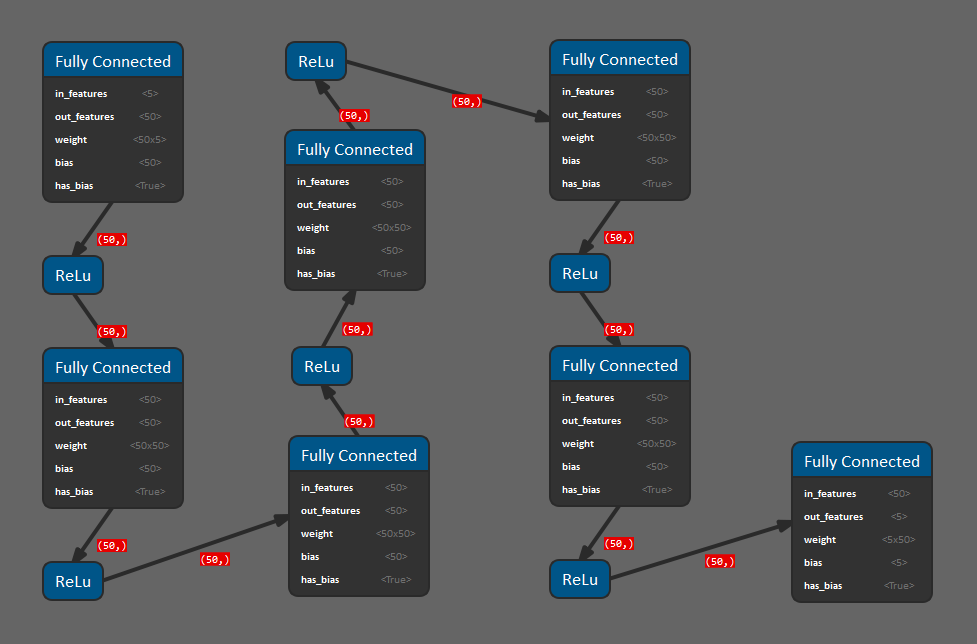
\includegraphics[width=1\textwidth]{imgs/ACAS_CCNN.png}
\label{img:acas-architecture}
\caption{Graphical representation of a ONNX model of an ACAS XU network. 
	The image is generated in \href{https://github.com/NeVerTools/NeVer2}
	{NeVer2}.}
\end{figure}

We consider a standard example of an ACAS XU network with 6 hidden
layers of 50 ReLU neurons each; the input and output layers consist 
of 5 neurons. In Figure~\ref{img:acas-architecture} we show a graphical
representation of this model. The ACAS XU network acts as a function 
$\nu : I^5 \to O^5$ with $I = O = \mathbb{R}$.  A property of interest 
for this kind of network can be stated as follows: 

\begin{equation}
\label{eq:acas-property1}
\begin{array}{l}
- \varepsilon_0 \leq x_0 \leq \varepsilon_0 \\
- \varepsilon_1 \leq x_1 \leq \varepsilon_1 \\
- \varepsilon_2 \leq x_2 \leq \varepsilon_2 \\
- \varepsilon_3 \leq x_3 \leq \varepsilon_3 \\
- \varepsilon_4 \leq x_4 \leq \varepsilon_4 \\
y_0 - y_1 \leq 0 \\
y_0 - y_2 \leq 0 \\
y_0 - y_3 \leq 0 \\
y_0 - y_4 \leq 0 \\
\end{array}
\end{equation}

where $\varepsilon_i \in \mathbb{R}+$ with $0 \leq i \leq 4$ are
arbitrary positive input noise constants, $(x_0, \ldots, x_4) 
\in \mathbb{R}^5$ is a sample of the input vector and 
$(y_0, \ldots, y_4) \in \mathbb{R}^5$ is the corresponding output
vector $(y_0, \ldots, y_4) = \nu((x_0, \ldots, x_4))$.

The property can be experessed in the SMT-LIB language using
specific identifiers for input and output vectors derived from
the identifiers used in the ONNX model. In particular, ONNX only
provides an identifier for the output of each layer and a global 
identifier for the network input; for this reason we identify the 
input tensor as $\mathbf{X}$ and the output tensor as the last 
Fully Connected (\textit{Gemm}) node identifier $\mathbf{FC6}$, 
both with dimension 5. We can then express property 
(\ref{eq:acas-property1}) in SMTLIB as:
\begin{lstlisting}
	
; definition of the variables of interest
(declare-fun X_0 () Real)
(declare-fun X_1 () Real)
(declare-fun X_2 () Real)
(declare-fun X_3 () Real)
(declare-fun X_4 () Real)

(declare-fun FC6_0 () Real)
(declare-fun FC6_1 () Real)
(declare-fun FC6_2 () Real)
(declare-fun FC6_3 () Real)
(declare-fun FC6_4 () Real)

; definition of the constraints
(assert (<= X_0 eps_0))
(assert (>= X_0 -eps_0))
(assert (<= X_1 eps_1))
(assert (>= X_1 -eps_1))
(assert (<= X_2 eps_2))
(assert (>= X_2 -eps_2))
(assert (<= X_3 eps_3))
(assert (>= X_3 -eps_3))
(assert (<= X_4 eps_4))
(assert (>= X_4 -eps_4))

(assert (<= (- FC6_0 FC6_1) 0.0))
(assert (<= (- FC6_0 FC6_2) 0.0))
(assert (<= (- FC6_0 FC6_3) 0.0))
(assert (<= (- FC6_0 FC6_4) 0.0))
\end{lstlisting}
This fragment of code is compliant with the SMT-LIB 2 language standard
and it defines the property of interest in term of input-output
relations.  Clearly, this code is not complete in terms of internal
constraints of the network: these will be extracted based on the
verification methodology of interest from the ONNX model of the network.

%%%%%%%%%%%%%%%%%%%%%%%%%
\section{MNIST}
%%%%%%%%%%%%%%%%%%%%%%%%%

\begin{figure}[t]
	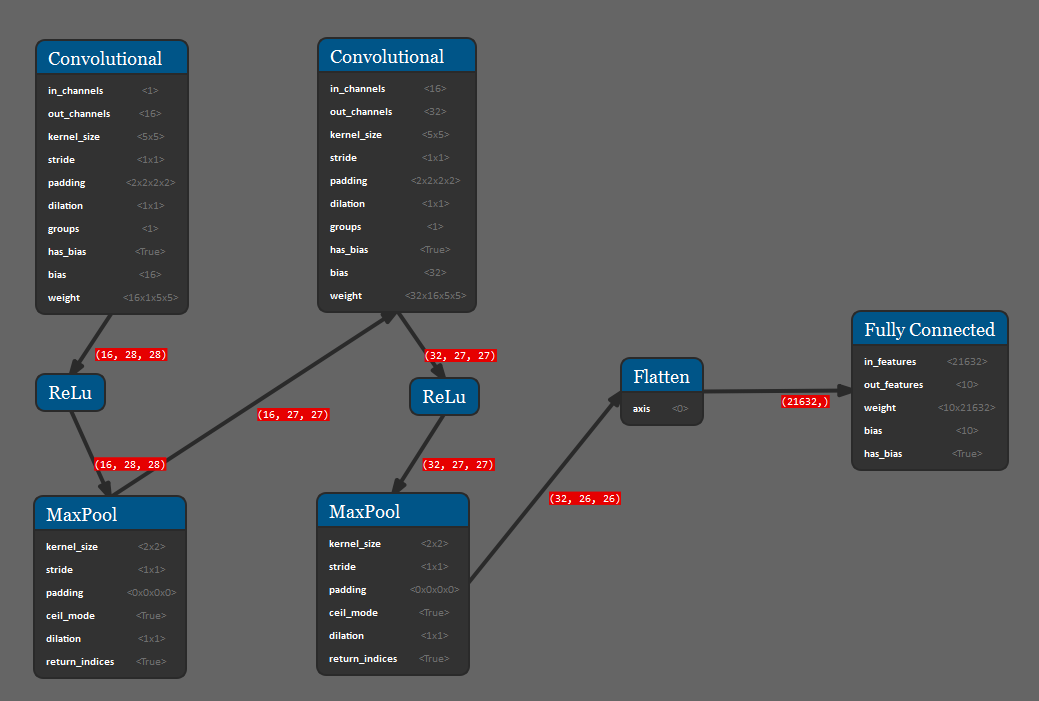
\includegraphics[width=1\textwidth]{imgs/MNIST_conv_CCNN.png}
	\label{img:mnist-architecture}
	\caption{Graphical representation of a ONNX model of a convolutional
		MNIST network. The image is generated in 
		\href{https://github.com/NeVerTools/NeVer2}{NeVer2}.}
\end{figure}

We consider a standard example of a convolutional MNIST network with 
two convolutional layers consisting of a convolution with a 5 $\times$ 5
kernel with 2 pixel padding, a ReLU activation function and a Max Pooling
with a 2 $\times$ 2 kernel. The first convolution generates 16 channels,
and the second 32; the result is flattened to a single vector which is
finally fed to a Fully Connected layer. The input layer consists of a 
three-dimensional tensor $1 \times 28 \times 28$ and the output layer 
consists of 10 neurons for the classification. 
In Figure~\ref{img:mnist-architecture} we show a graphical
representation of this model. A network for classifying objects in the MNIST
dataset is a function $\nu : I^{1,28,28} \to O^{10}$ with $I = O = \mathbb{R}$.

A local robustness property can be expressed in a similar way with respect
to the ACAS XU network: for a local sample $\hat{x}$ such that 
$\nu(\hat{x}) = y_9$ and an input noise $\varepsilon$, the classification 
should not change for a $\varepsilon$ perturbation.

\begin{equation}
	\label{eq:mnist-property1}
	\begin{array}{l}
		\forall i \in [0, 783] : 
			\hat{x} - \varepsilon \leq x_i \leq \hat{x} + \varepsilon \\	
		\forall j \in [0, 8] : y_j - y_9 \leq 0
	\end{array}
\end{equation}

In order to represent correctly the variables corresponding to multi-dimensional
tensors we allow two different notations: one that distinguishes the 
single dimensions and one that flattens the tensor in a single 1-D array.

\paragraph{Tensor representation.}
Let $x^D$ be a tensor in a $D$-dimensional space. We associate the dimensional
subscripting with a single underscore for separating the variable name and the
variable subscript, and $D-1$ dashes for separating the dimension values:
\begin{itemize}
	\item \textit{1-D} tensor: X\_0, X\_1, \ldots, X\_n
	\item \textit{2-D} tensor: X\_0-0, X\_0-1, \ldots, X\_1-0, X\_1-1, \ldots, X\_n-m
	\item \textit{3-D} tensor: X\_0-0-0, \ldots, X\_i-j-k, \ldots, X\_n-m-p
	\item $\cdots$
\end{itemize}
In the example above, X\_0-3-2 corresponds to the input $x_{0,3,2} \in x^3$ in 
tensor form.
\myremark{Please note that this notation is encouraged, as it provides a clearer
interpretation of the property.}

\paragraph{Array representation.}
Let $x^D$ be a tensor in a $D$-dimensional space. We provide the following
algorithm to flatten it in a single 1-$D$ array.
\begin{algorithm}
	\caption{Tensor flattening}
	\label{alg:flatten}
	\begin{algorithmic}[1]
		\Procedure{flatten}{$x$}
			\State $idx = 0$
			\For{$a == 0$ to $N_1$}
				\For{$b == 0$ to $N_2$}
					\State $\ldots$
					\For{$k == 0$ to $N_k$}
						\State X\_$idx$ = $x_{a, b, \ldots, k}$
						\State $idx = idx + 1$
					\EndFor
				\EndFor
			\EndFor
		\EndProcedure
	\end{algorithmic}
\end{algorithm}

All properties which comply with either representation should be accepted
and readable. An example in the SMT-LIB language is provided as follows,
highlighting the two possibilities for defining the variables.

\begin{lstlisting}
	
; definition of the variables of interest
(declare-fun X_0 () Real) ; (declare-fun X_0-0-0 () Real)
(declare-fun X_1 () Real)
(declare-fun X_2 () Real)
...
(declare-fun X_782 () Real) ; (declare-fun X_0-26-27 () Real)
(declare-fun X_783 () Real) ; (declare-fun X_0-27-27 () Real)

(declare-fun FC0_0 () Real)
(declare-fun FC0_1 () Real)
(declare-fun FC0_2 () Real)
...
(declare-fun FC0_9 () Real)

; definition of the constraints
(assert (<= X_0 eps)) ; (assert (<= X_0-0-0 eps))
(assert (>= X_0 -eps)) ; (assert (>= X_0-0-0 -eps))
...
(assert (<= X_783 eps)) ; (assert (<= X_0-27-27 eps))
(assert (>= X_783 -eps)) ; (assert (>= X_0-27-27 -eps))

(assert (<= (- FC0_0 FC0_9) 0.0))
(assert (<= (- FC0_1 FC0_9) 0.0))
...
(assert (<= (- FC0_8 FC0_9) 0.0))
\end{lstlisting}

\end{document}
